\documentclass[12pt,a4paper]{article}

\usepackage[UTF8]{ctex}
\usepackage{geometry}
\usepackage{graphicx}
\usepackage{booktabs}
\usepackage{hyperref}
\usepackage{setspace}
\usepackage{float}
\usepackage{caption}

\geometry{left=2.5cm,right=2.5cm,top=2.5cm,bottom=2.5cm}
\onehalfspacing
\graphicspath{{figures/}}

\title{穿行于多个澳门：城市空间如何翻译文化身份\\
\large Walking Through Many Macaus: How Urban Spaces Translate Cultural Identity}
\author{UCUG1600 跨文化交流 Final Report\\小组成员：待填写}
\date{\today}

\begin{document}
\maketitle

\begin{abstract}
本文基于一次澳门 field trip 的照片、视频和现场观察，探讨澳门城市空间如何通过语言、建筑、声音、消费符号和移动路线呈现多重文化身份。调查前，我们使用 AI 作为头脑风暴工具，获得了“双名街道”和“声音地图”两个初始方向；但在整理真实素材后，我们发现单一路牌或声音主题不足以解释整个路线中的观察。因此，本文将研究焦点扩展为“城市空间如何翻译文化身份”。报告分析四类空间：口岸与交通空间、历史遗产空间、日常街道空间、全球消费景观。研究认为，澳门的跨文化交流并不只存在于双语路牌或历史建筑中，而是在人的移动过程中被不断体验和重新解释。换言之，澳门不是一个故事被翻译成两种语言，而是多个文化故事在同一条路线中被不断切换、观看和参与。
\end{abstract}

\section{Introduction}

澳门常被概括为“中西文化融合”的城市。这一说法并非错误，但如果只停留在宏观标签上，就容易把澳门的跨文化经验简化为几个固定符号：葡式建筑、中文和葡文路牌、赌场、手信街或世界遗产。我们的 field trip 让我们意识到，澳门的跨文化性不是静止地摆在某一个景点或某一块路牌上，而是在人的移动过程中逐步出现。

我们从口岸进入澳门，经过大巴和酒店娱乐场，再进入大三巴周边街道、圣物宝库和大炮台，最后到达威尼斯人和澳门官方 NBA 店。沿途的照片和视频显示，同一座城市在不同空间中呈现出明显不同的文化身份：口岸体现边境和制度秩序；大三巴和大炮台体现宗教遗产、殖民记忆和旅游叙事；大三巴周边街道体现日常商业、招牌和人流；威尼斯人和 NBA 店则体现全球消费文化和被设计出来的国际化体验。

因此，本文不把本次 field trip 写成旅游记录，而是把路线本身作为研究框架。我们的核心问题是：澳门的城市空间如何通过语言、建筑、声音、消费符号和移动路线呈现多重文化身份？

\section{Research Question}

本文的主研究问题是：

\begin{quote}
澳门的城市空间如何通过语言、建筑、声音、消费符号和移动路线呈现多重文化身份？
\end{quote}

英文表述为：

\begin{quote}
How do Macau's urban spaces communicate multiple cultural identities through language, architecture, sound, consumer symbols, and movement?
\end{quote}

该问题可以进一步拆分为三个子问题：

\begin{enumerate}
  \item 不同空间如何让我们感受到不同的“澳门”？
  \item 这些空间如何体现跨文化交流中的语言与非语言符号？
  \item 实地观察如何修正 AI 在调查前给出的研究设想？
\end{enumerate}

\section{Conceptual Framework}

\subsection{Self and Other}

跨文化交流中的“自我”与“他者”并不是固定不变的身份，而是在具体场景中被建构出来的关系。口岸空间尤其能体现这一点。通关、排队、证件检查、导向牌和接驳交通让进入者意识到：自己正在从熟悉的社会空间进入另一个制度空间。这里的跨文化交流并不一定表现为人与人之间的对话，而是表现为边境秩序对身体移动的组织。

这一概念对应课程 ILO\#1，即理解“自我与他人”的概念以及文化意识在跨文化交流中的作用。在本项目中，口岸并不是无关紧要的转场，而是我们接触到的第一个“澳门”。

\subsection{Linguistic Landscape}

语言景观（linguistic landscape）通常指公共空间中可见语言的分布和使用，例如街名、路牌、招牌、菜单、广告和店铺标识。调查前，AI 曾建议我们研究澳门中葡街名之间的“不对等翻译”。这一方向有价值，因为澳门街名确实体现了不同文化系统对同一空间的命名权和解释权。

不过，实地观察后我们发现，语言景观不只存在于路牌中，也存在于大三巴周边的手信店、小吃街、菜单、游客导向和商品陈列中。因此，本文保留“语言景观”的视角，但不把研究限制在街名翻译上。我们更关注公共空间如何通过多种符号共同讲述澳门。

\subsection{Non-verbal Communication and Sensory Observation}

课程强调语言与非语言交流能力。我们的素材显示，很多跨文化信息并不是通过文字表达的，而是通过空间秩序、声音氛围、建筑风格、灯光、商场动线和身体参与传递的。例如，口岸的排队栏杆和广播构成秩序感；威尼斯人通过穹顶、运河和灯光制造“欧洲想象”；NBA 店通过电子屏和投篮互动让消费者参与美国体育文化。

因此，本文把声音和氛围作为辅助观察维度。我们没有进行系统录音，所以不会把它包装成完整的 soundscape study；但声音确实帮助我们区分不同空间，例如口岸的广播、人群脚步，历史街区的游客语言和店铺声音，威尼斯人和 NBA 店的室内音乐与电子游戏声。

\subsection{Space as Storytelling}

城市空间本身具有 storytelling 的功能。大三巴通过石构立面、宗教遗迹和游客观看方式讲述“遗产澳门”；威尼斯人通过模拟欧洲建筑和室内运河讲述“全球消费澳门”；NBA 店通过球衣、屏幕和互动游戏讲述“全球流行文化澳门”。这些空间不是中立背景，而是主动组织观众理解澳门的方式。

这对应课程 ILO\#4，即面向国际观众培养具有文化意识的讲故事能力。本项目的 presentation 也采用“跟着路线移动”的方式，让观众体验多个文化故事如何在同一座城市中切换。

\section{Methodology}

\subsection{Field Site and Route}

本次 field trip 的主要路线为：口岸/通关空间 → 大巴与酒店娱乐场 → 大三巴周边街道 → 大三巴、圣物宝库和大炮台 → 公交/交通转场 → 威尼斯人与澳门官方 NBA 店 → 返程。这个路线后来成为我们的分析框架，因为每一次地点转换都带来一种新的文化解释框架。

\subsection{Data Collection}

本项目使用以下方法收集材料：

\begin{itemize}
  \item Direct observation / 直接观察；
  \item Photo and video documentation / 照片与视频记录；
  \item Walking route analysis / 路线分析；
  \item Sensory notes / 声音与氛围观察。
\end{itemize}

我们没有进行正式访谈，因此本文不声称代表澳门居民、游客或商家的主观观点。我们的分析集中于公共空间中可观察到的语言、建筑、声音、动线和消费符号。这样的设计与 Fieldwork Tutorial 中关于 direct observation 和 recording observations 的方法要求一致。

\subsection{Fieldwork Ethics}

本项目主要记录公共空间。我们在分析时尽量避免把陌生个体作为研究对象，而是关注空间、符号和场景本身。对于出现人群的图片和视频，我们只把它们作为公共空间使用方式的证据，例如游客凝视、人流动线或排队秩序。我们也避免把澳门简单化为“中西融合”的刻板结论，而是承认不同空间中存在不同层次的文化叙事。

\subsection{AI Use}

AI 在本项目中作为前期头脑风暴工具。它提供了“双名街道”和“声音地图”两个可能方向。实地调查后，我们根据真实素材对研究焦点进行了修正，并最终形成“城市空间如何翻译文化身份”的框架。换言之，AI 提供的是入口，而不是最终答案；最终分析来自我们自己的 fieldwork 素材、路线观察和小组讨论。

\section{Findings}

\subsection{Macau as Border: Entering a Cultural Order}

我们最先接触到的澳门不是大三巴，也不是威尼斯人，而是口岸大厅、排队栏杆、导向牌、通关流程和接驳大巴。这个空间通过非语言方式组织人的身体移动：人们沿着栏杆排队，跟随导向牌前进，完成通关后再进入交通接驳区。

\begin{figure}[H]
  \centering
  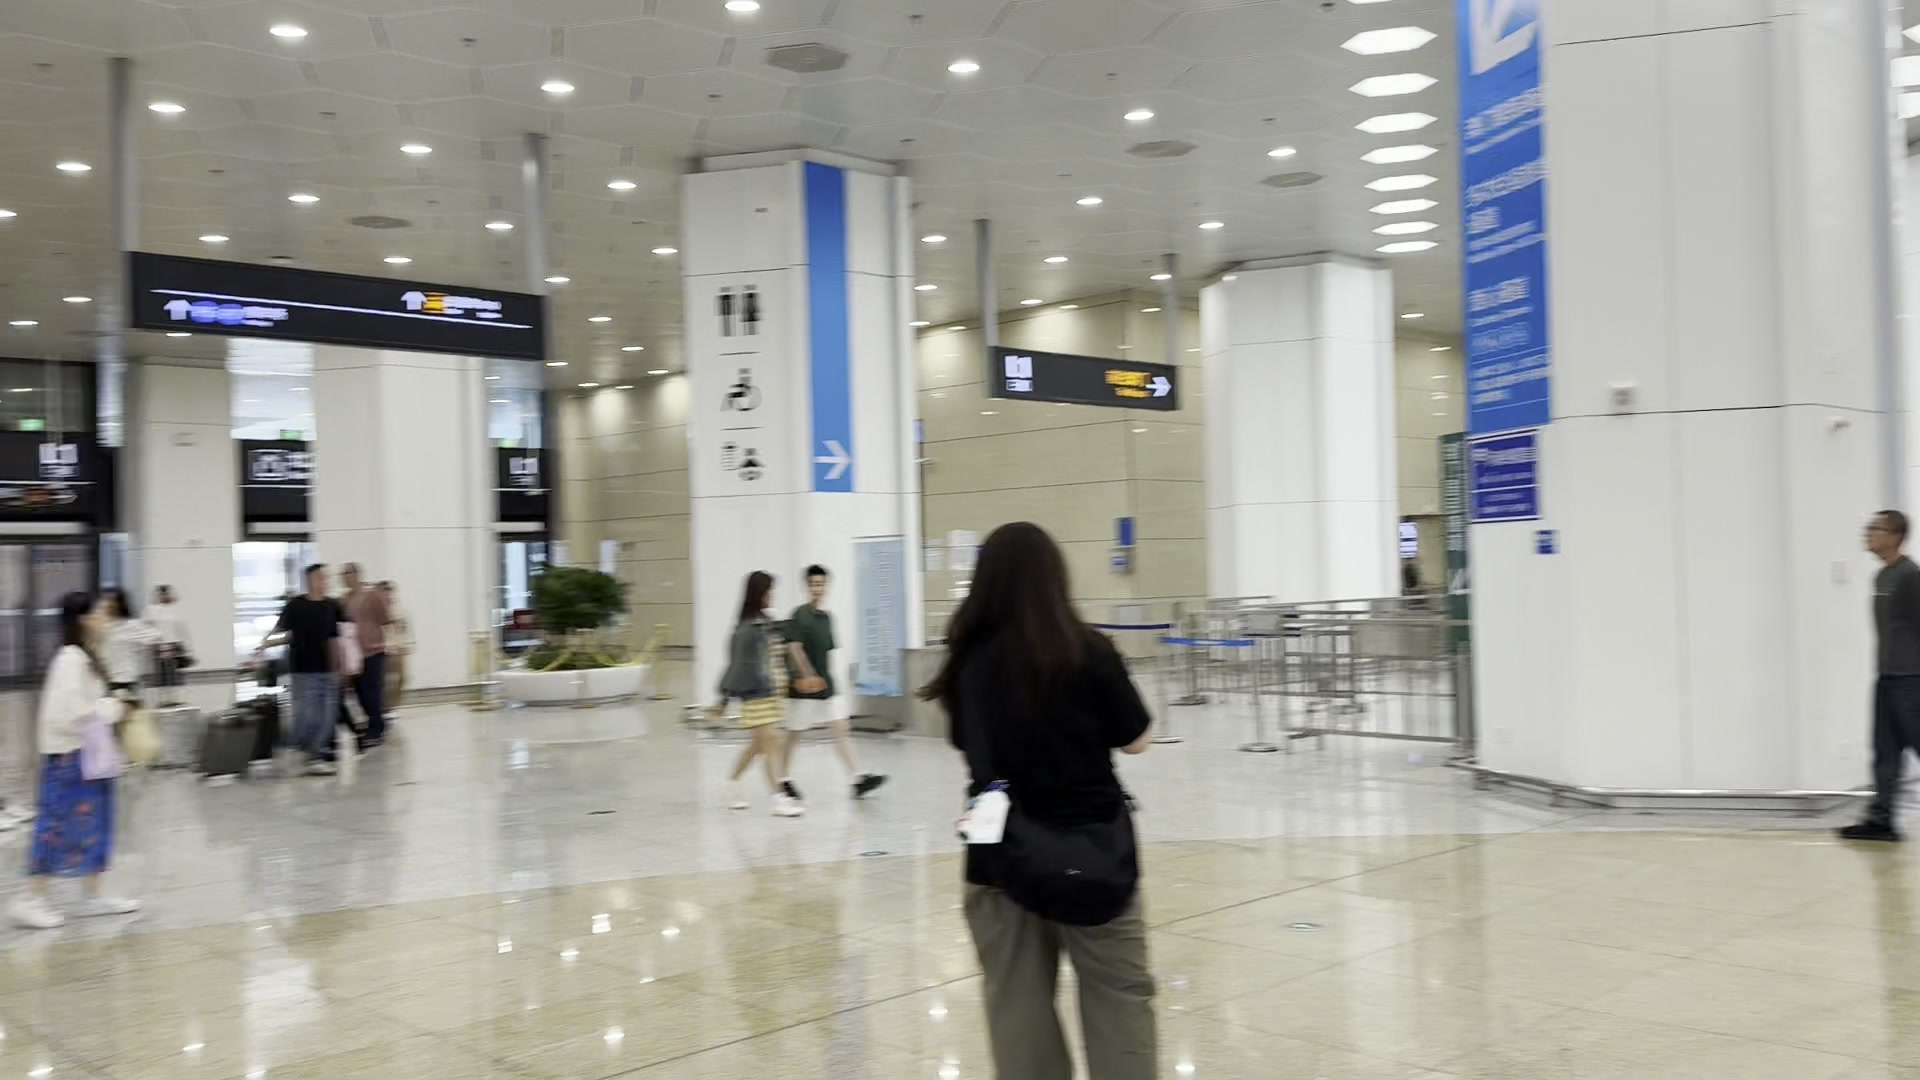
\includegraphics[width=0.82\linewidth]{fig1_border.jpg}
  \caption{口岸大厅中的导向、通行空间和人群移动。}
\end{figure}

这一发现说明，进入澳门本身就是一种跨文化体验。边境空间让“自我”和“他者空间”的关系变得具体：我们从原来的日常空间进入另一个制度空间，并通过排队、证件、导向和交通完成身份与空间的转换。这种转换不依赖长篇语言说明，而是通过空间秩序和身体行为完成。

\subsection{Macau as Heritage: Religion, Colonial Memory, and Tourism}

第二个澳门是作为历史遗产的澳门。大三巴牌坊是澳门最容易被识别的视觉符号之一。它把澳门呈现为天主教、葡萄牙殖民历史和世界遗产的空间。但现场的人流、拍照和游客移动也提醒我们：遗产不是沉默的历史，它在今天被不断观看、消费和重新讲述。

\begin{figure}[H]
  \centering
  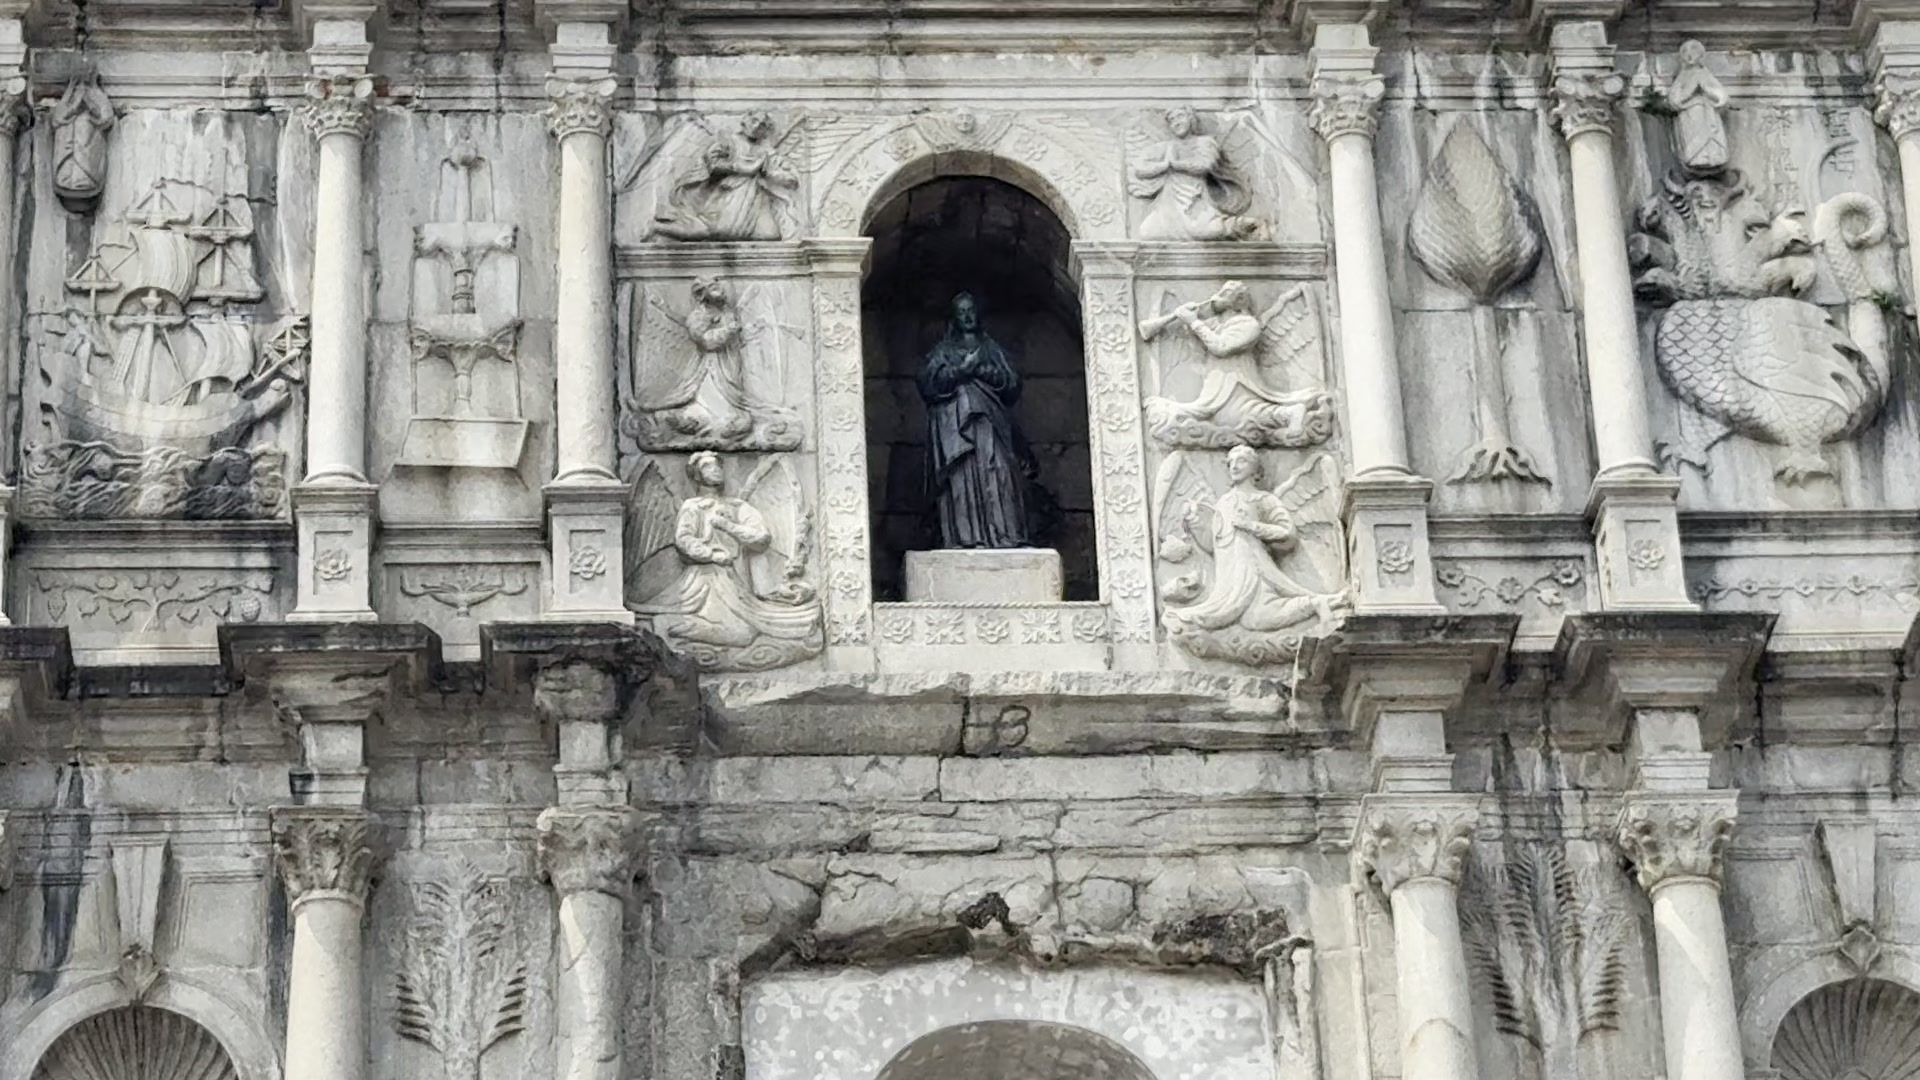
\includegraphics[width=0.82\linewidth]{fig2_ruins.jpg}
  \caption{大三巴牌坊石构细节：遗产空间以建筑符号讲述宗教与殖民历史。}
\end{figure}

圣物宝库与墓室进一步说明，大三巴不只是适合拍照的立面，也连接着宗教记忆。展区标识、墓室空间和宗教展陈让游客进入更具体的天主教历史叙事。

\begin{figure}[H]
  \centering
  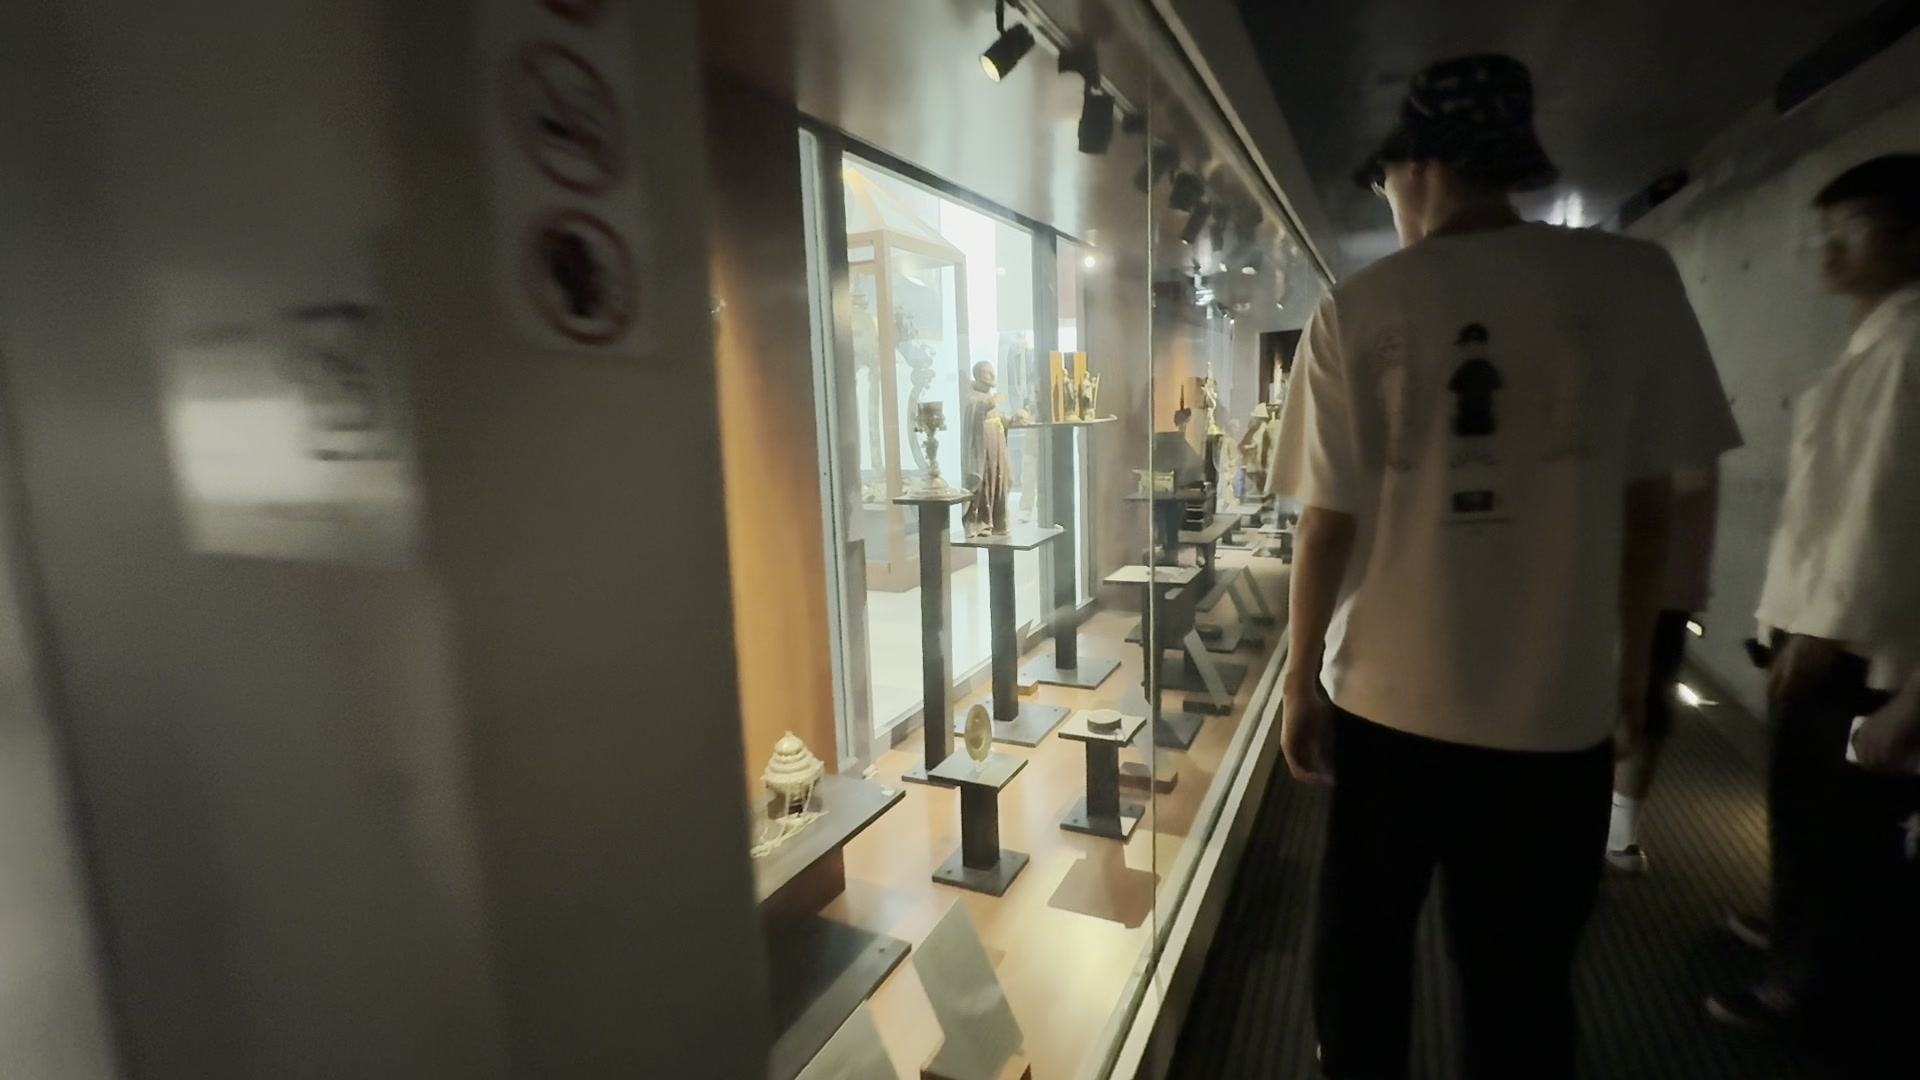
\includegraphics[width=0.82\linewidth]{fig3_crypt.jpg}
  \caption{圣物宝库与墓室将景点视觉转化为宗教记忆。}
\end{figure}

大炮台则提供了另一个视角。站在历史遗址上俯瞰现代城市时，历史和现代同时出现在同一个画面中。这个视角让我们看到，澳门的历史遗产并没有与当代城市生活分离，而是成为观察现代澳门的一个平台。

\begin{figure}[H]
  \centering
  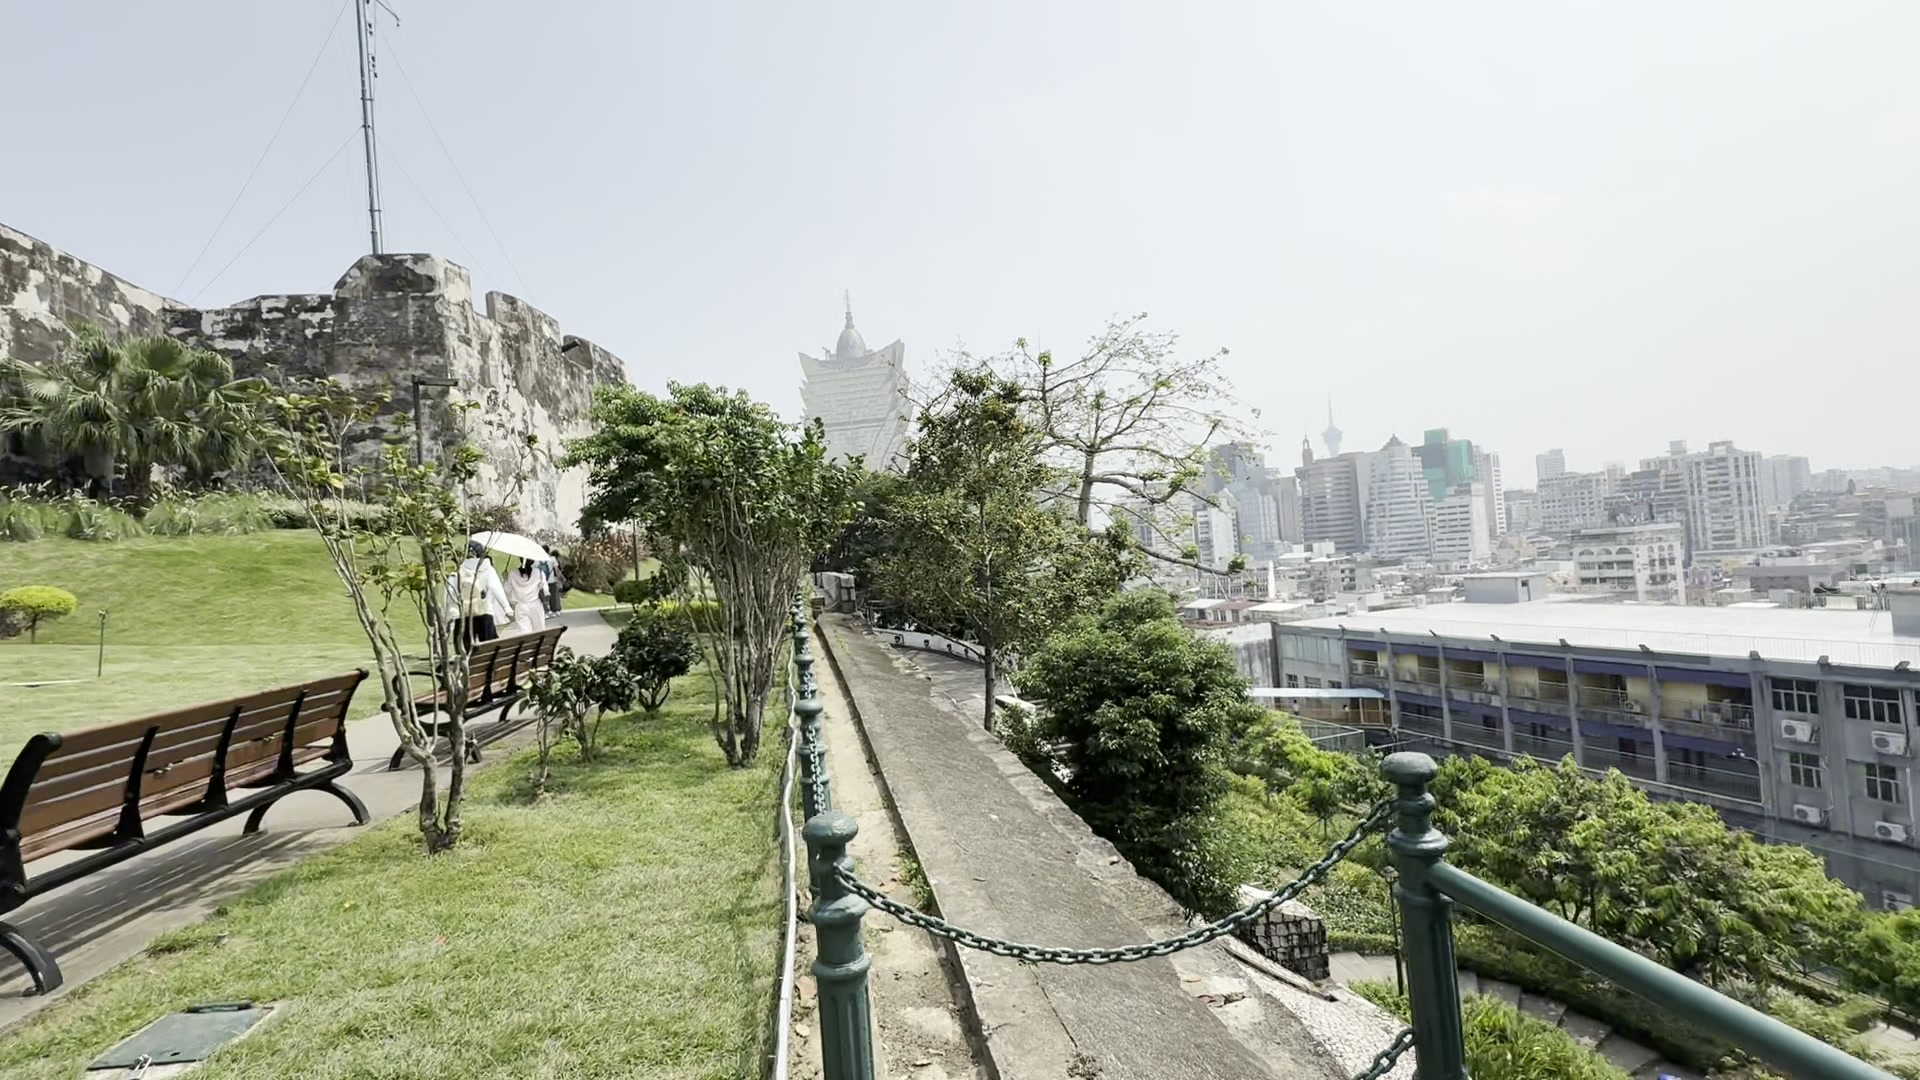
\includegraphics[width=0.82\linewidth]{fig4_fort_view.jpg}
  \caption{从大炮台俯瞰城市：历史遗址与现代景观同框。}
\end{figure}

\subsection{Macau as Everyday Street: Language, Signs, and Commercial Life}

第三个澳门是作为日常街道的澳门。大三巴周边并不只有宏大的历史遗产，也有小吃街、手信店、密集招牌、人流和餐饮空间。这里的文化交流更日常，也更商业化。

\begin{figure}[H]
  \centering
  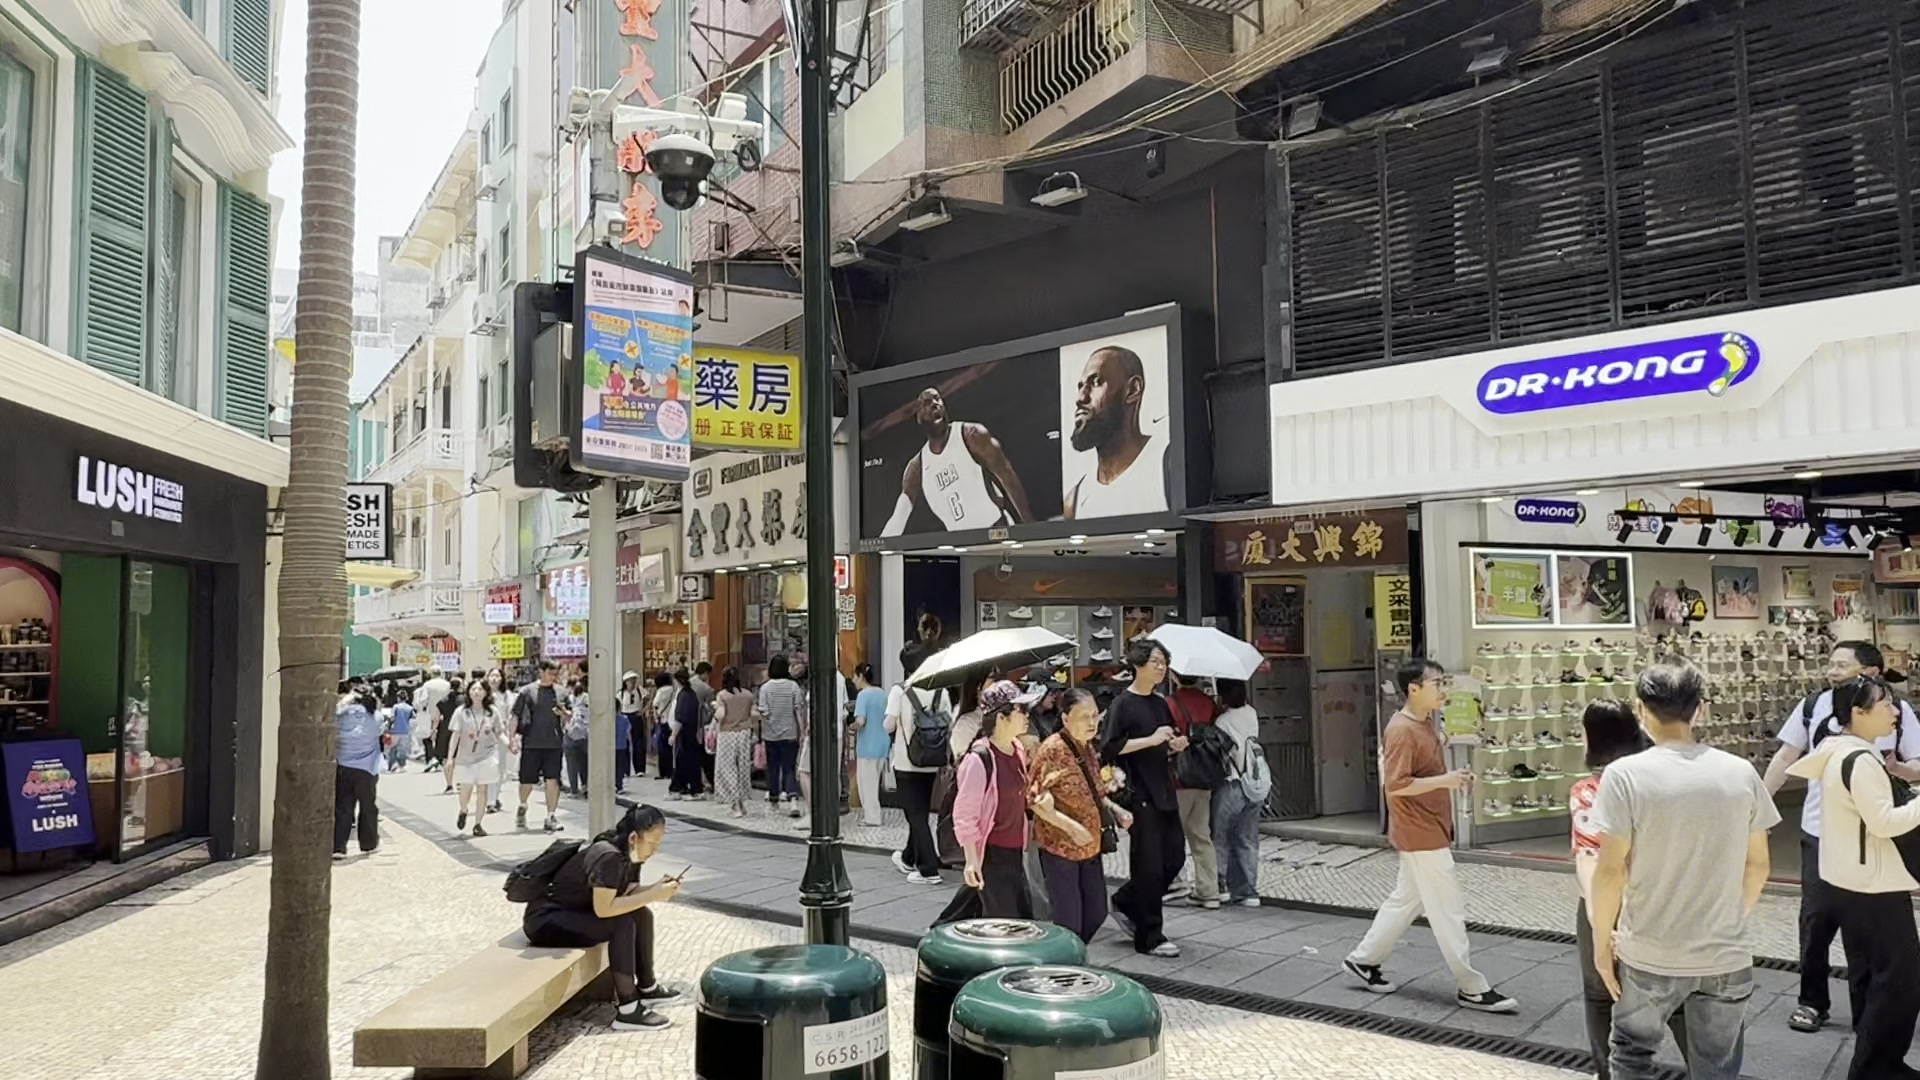
\includegraphics[width=0.82\linewidth]{fig5_street.jpg}
  \caption{大三巴周边街道中的招牌、人流和商业空间。}
\end{figure}

AI 一开始提醒我们注意“双名街道”，也就是中葡街名之间的语义错位。实地观察让我们意识到，语言景观不只存在于路牌中，也存在于招牌、菜单、商品陈列和游客移动中。大三巴周边的街道把历史遗产和日常商业连接起来：游客从商业街走向地标，地标又反过来吸引商业活动。这种空间关系让澳门同时呈现为遗产城市和旅游消费城市。

\subsection{Macau as Global Spectacle: Venetian, Gaming, and NBA}

第四个澳门是作为全球景观的澳门。威尼斯人、酒店娱乐场和 NBA 店展示了另一种文化身份：这里的跨文化交流不再主要依赖中葡历史，而是通过全球品牌、模拟建筑和消费体验发生。

威尼斯人通过欧洲式外立面、室内穹顶、运河、灯光和商场动线制造出一种“在澳门内部的欧洲想象”。它和大三巴形成了鲜明对比：大三巴是历史留下来的遗产，而威尼斯人是商业设计出来的“遗产感”和“欧洲感”。

\begin{figure}[H]
  \centering
  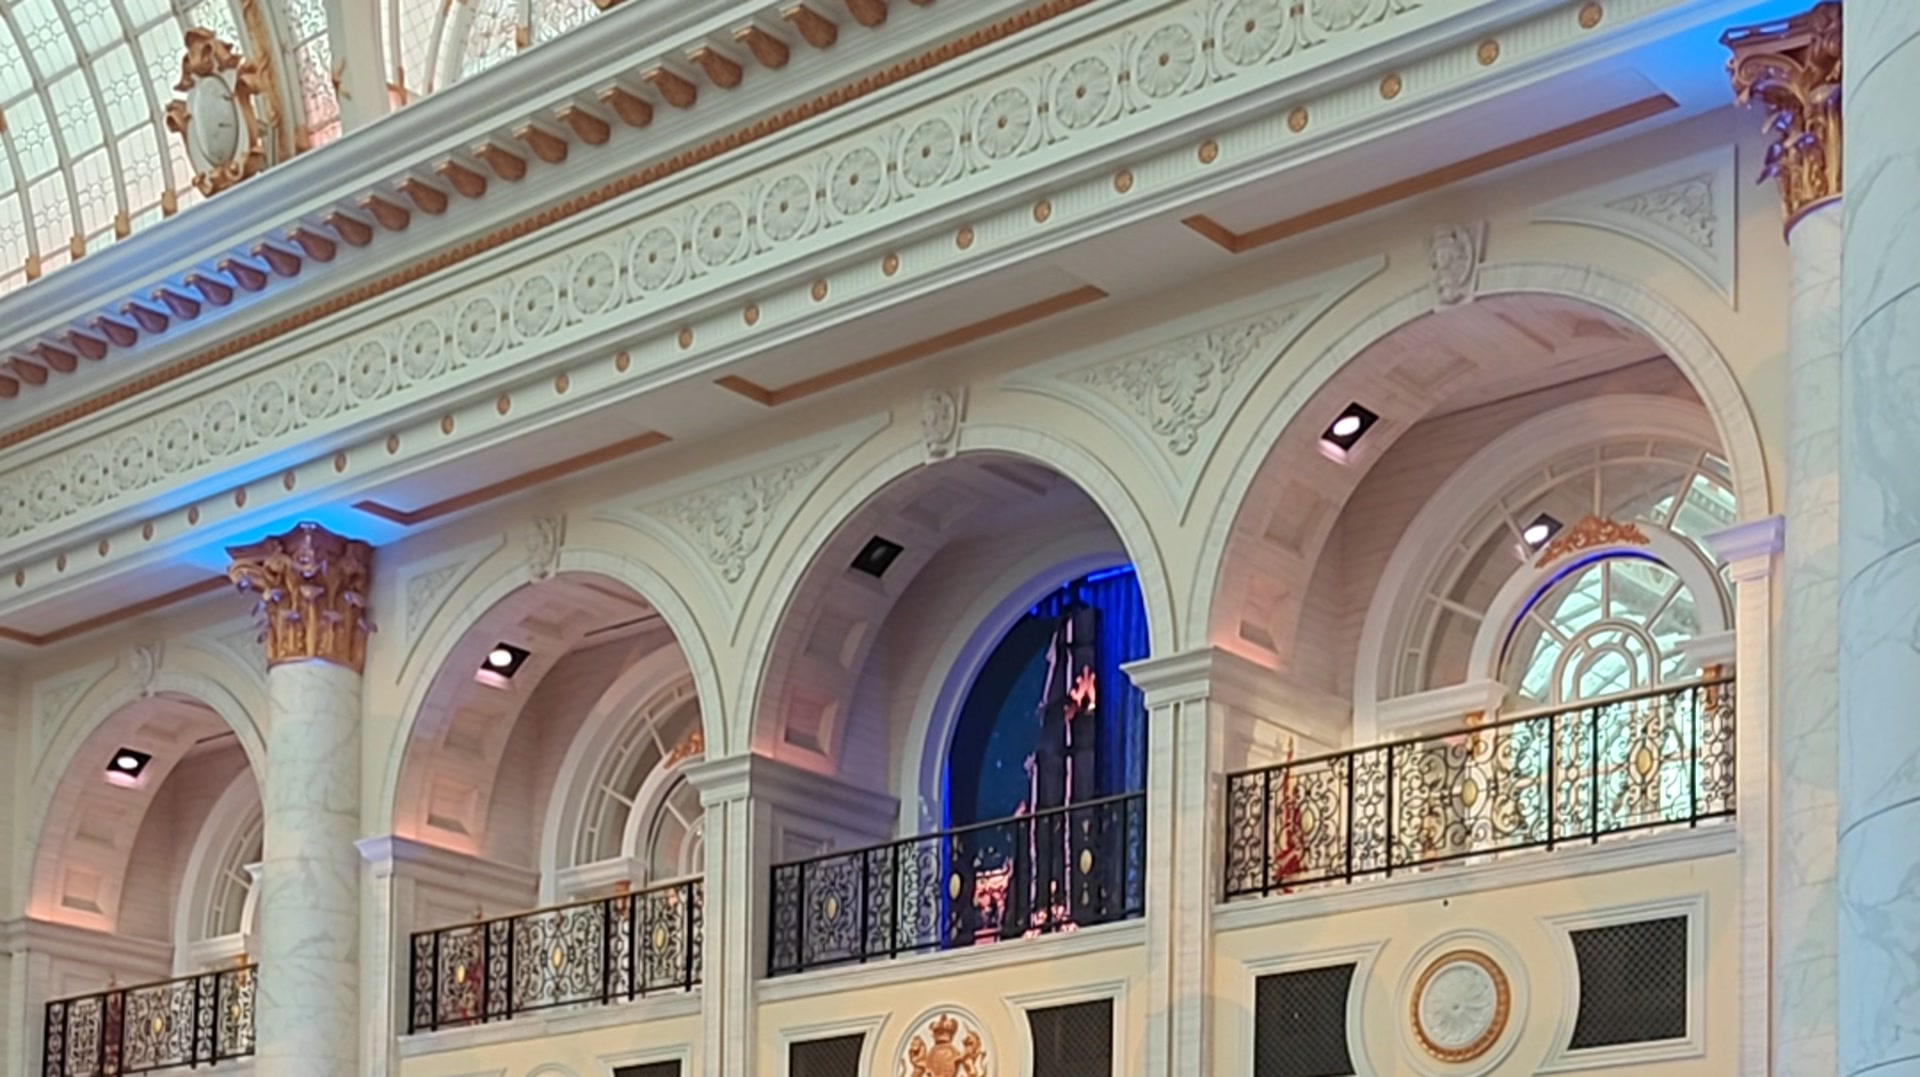
\includegraphics[width=0.82\linewidth]{fig6_venetian.jpg}
  \caption{威尼斯人多层商场立面、拱窗和时钟装饰制造出被设计的欧洲想象。}
\end{figure}

澳门官方 NBA 店进一步说明，跨文化交流不只发生在传统文化或历史遗产中，也发生在全球流行文化中。美国体育文化在这里被商品化、游戏化，并通过投篮互动让身体参与进去。球衣、电子屏、计分系统和投篮动作共同构成一种参与式的跨文化消费体验。

\begin{figure}[H]
  \centering
  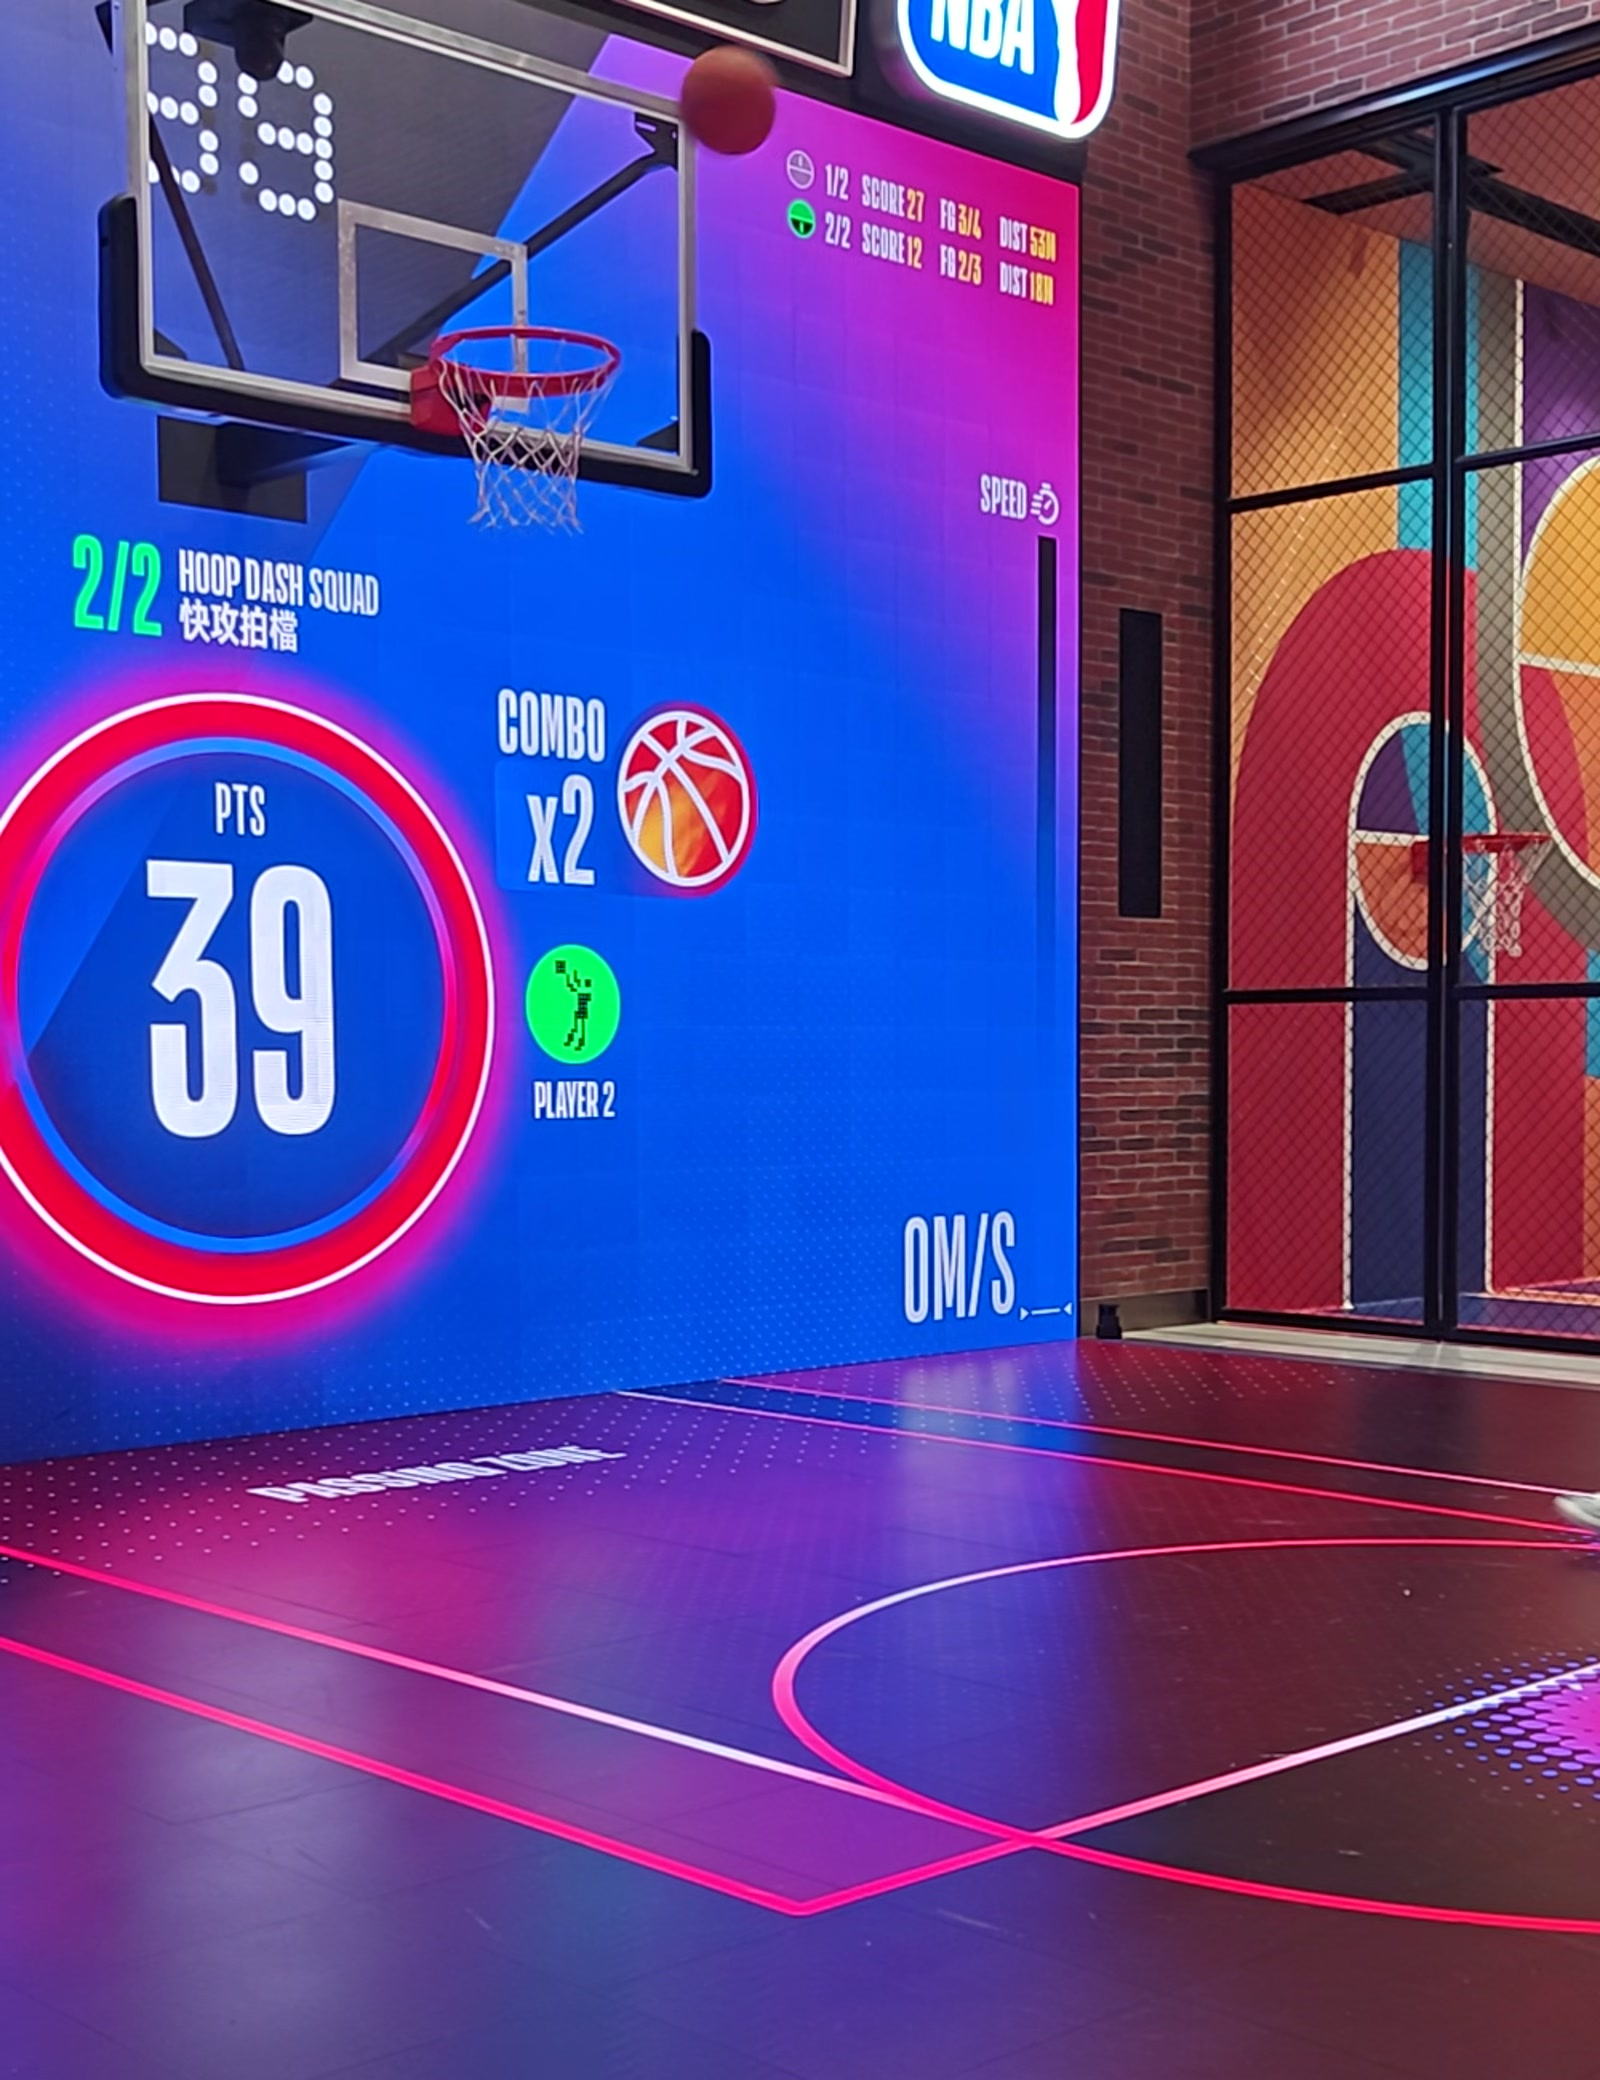
\includegraphics[width=0.82\linewidth]{fig7_nba.jpg}
  \caption{NBA 店互动体验区：分数、篮筐和屏幕反馈把全球体育文化转化为可参与的游戏化体验。}
\end{figure}

\section{Discussion}

\subsection{From Cultural Fusion to Spatial Switching}

如果只用“中西融合”概括澳门，就会忽略不同空间之间的差异。我们的 fieldwork 更适合用 spatial switching 来解释：人在移动中不断切换文化解释框架。口岸让澳门成为边境城市；大三巴和大炮台让澳门成为历史遗产空间；大三巴周边街道让澳门成为日常商业空间；威尼斯人和 NBA 店让澳门成为全球消费景观。

这种切换说明，澳门的跨文化交流不是单一文化混合后的稳定结果，而是多个文化叙事在不同空间中被激活。观众、游客或学生每进入一个新空间，就会被引导去理解一个新的澳门。

\subsection{Translation Beyond Language}

本项目标题中的“translate”并不只指中文和葡文之间的语言翻译。它也指空间如何把澳门翻译成不同身份。口岸通过秩序和通关流程翻译澳门；大三巴通过宗教遗产和游客凝视翻译澳门；街道通过招牌、小吃和人流翻译澳门；威尼斯人和 NBA 店通过全球品牌和消费互动翻译澳门。

因此，跨文化交流可以被理解为一种空间翻译。不同空间不是简单承载文化，而是在主动组织文化意义。

\subsection{What Fieldwork Changed}

AI 给出的“双名街道”和“声音地图”方向为我们提供了有价值的入口，但 fieldwork 改变了我们的研究问题。如果我们强行只讲街名，会浪费口岸、大三巴、大炮台、威尼斯人和 NBA 店这些重要素材；如果强行只讲声音，又会夸大我们并没有系统录音的部分。

因此，我们选择用实地材料修正 AI 主题。这一点本身也体现了课程所强调的批判性思维：AI 可以帮助提出问题，但不能代替真实观察。最终的研究框架必须从现场材料中生长出来。

\section{Limitations}

本项目有几个局限。第一，我们没有进行正式访谈，因此不能代表澳门居民、游客或商家的主观经验。第二，声音观察不是系统录音研究，只作为 sensory layer 辅助分析。第三，路线覆盖有限，主要集中在口岸、历史城区和路氹商业区，不能代表澳门所有社区。第四，素材来自一次 field trip，时间跨度较短。第五，部分地点判断依赖照片、视频和路线记忆，细节上可能不完整。

这些局限并不否定本研究的价值，而是说明本文的结论应被理解为一次基于公共空间观察的 fieldwork analysis，而不是关于澳门整体社会文化的完整民族志研究。

\section{Conclusion}

本文认为，澳门的跨文化交流并不只存在于双语路牌或历史建筑中，而是在人的移动过程中被不断体验和重新解释。我们从口岸进入澳门，穿过历史城区和商业街道，最后到达威尼斯人和 NBA 店；沿途看到的不是一个单一澳门，而是多个文化身份不断切换的澳门。

因此，澳门不是一个故事被翻译成两种语言，而是多个文化故事在人的移动中被不断体验。对我们来说，这次 fieldwork 的价值不在于证明 AI 一开始给出的题目，而在于通过真实观察修正它。跨文化交流不只发生在语言翻译或面对面对话中，也发生在城市空间、视觉符号、声音氛围和消费实践中。

\appendix
\section{Selected Media Inventory}

\begin{table}[H]
\centering
\caption{精选素材与分析功能}
\begin{tabular}{p{0.18\linewidth}p{0.34\linewidth}p{0.36\linewidth}}
\toprule
空间类型 & 代表素材 & 分析功能 \\
\midrule
Border Macau & 口岸大厅、排队区、接驳大巴 & self/other、非语言秩序、跨境移动 \\
Heritage Macau & 大三巴、圣物宝库、大炮台 & 宗教记忆、殖民历史、游客凝视 \\
Everyday Street Macau & 大三巴周边街道、招牌、小吃街 & 语言景观、日常商业、旅游街道经验 \\
Global Spectacle Macau & 威尼斯人、酒店娱乐场、NBA 店 & 全球消费文化、模拟欧洲、美国体育文化 \\
\bottomrule
\end{tabular}
\end{table}

\section{References}

\begin{itemize}
  \item Hall, E. T. \& Hall, M. R. (2016). \textit{The Silent Language}. Course recommended reading.
  \item Scollon, R., Scollon, S. W., \& Jones, R. H. (2011). \textit{Intercultural Communication: A Discourse Approach}. Wiley.
  \item Samovar, L. A. et al. (2014). \textit{Intercultural Communication: A Reader}. Cengage Learning.
  \item UCUG1600 Course Syllabus and Fieldwork Tutorial materials.
\end{itemize}

\end{document}
